\documentclass[]{article}

\usepackage[utf8]{inputenc}
\usepackage[english,serbian]{babel}
\usepackage[margin=0.7in]{geometry}
\usepackage{url}
\usepackage{float}
\usepackage[graphicx]{realboxes}
\usepackage{listings}
\usepackage{textcomp}
\usepackage{xcolor}
\usepackage{titlesec}
\usepackage{adjustbox}
\lstset {
    language=HTML,
    frame=none,
    %xleftmargin=-.25in,
    %xrightmargin=.25in
    framesep=10pt,
    tabsize=4,
    showstringspaces=false,
    upquote=true,
    commentstyle=\color{black},
    keywordstyle=\color{black},
    stringstyle=\color{black},
    basicstyle=\small\ttfamily,
    emph={int,char,double,float,unsigned,void,bool},
    emphstyle={\color{black}},
    escapechar=\&,
    classoffset=1,
    morekeywords={>,<,.,;,,,-,!,=,~},
    keywordstyle=\color{black},
    classoffset=0,
    breaklines=true
}
\pagenumbering{gobble}

\titlespacing\title{left spacing}{before spacing}{after spacing}[right]

\title{Ra\v{c}unarske mre\v{z}e 4I, Ispit - Jun 1}
\date{05.06.2019.}

\begin{document}

\makeatletter
\begin{center}

{\fontsize{12pt}{14pt}\selectfont\bfseries\@title\par}
\@date

Pro\v{c}itati sve zadatke \textbf{pa\v{z}ljivo} pre rada - sve \v{s}to nije navedeno ne mora da se implementira! 

Vreme za rad: \textbf{2.5h}. Sre\'{c}no!
\end{center}
\makeatother


\begin{enumerate}
  \item Sockets \textbf{(15p)}
  \begin{itemize}
    \item Napraviti Java aplikaciju koja ima ulogu chat klijenta. Povezati se na lokalni server na portu 12345 koriste\'c{}i \texttt{Socket} klasu i ispisati sadr\v{z}aj koji server \v{s}alje nazad. Omogu\'c{}iti da klijent mo\v{z}e slati sadr\v{z}aj sa standardnog ulaza serveru (liniju po liniju). \hfill (3p)
    \item Napraviti Java aplikaciju koja ima ulogu pojednostavljenog chat servera. Pokrenuti lokalni server na portu 12345 koriste\'c{}i \texttt{ServerSocket} klasu. Server svim povezanim klijentima prosledjuje poruke pristigle od bilo kog klijenta. Prilikom povezivanja na server svaki klijent dobija svoj ID i obradjuje se u zasebnoj niti pri \v{c}emu se svim ostalim klijentima se prvo \v{s}alje ID pristiglog klijenta. Kad god neki klijent po\v{s}alje poruku, ista se prosledjuje svim ostalim klijentima. \hfill (10p)
    \item Poslati svim klijentima poruku u slu\v{c}aju da neki klijent prekine vezu (npr \texttt{Klijent <id> je napustio chat.}). \hfill (1p)
    \item Postarati se da su svi resursi ispravno zatvoreni u slu\v{c}aju izuzetka. \hfill (1p)
  \end{itemize}

  \item Swing \textbf{(15p)}
  Napraviti Java Swing aplikaciju koja ima ulogu jednostavnog HTML editora. Izgled aplikacije i HTML test primer su dati na slede\'c{}oj strani.
  \begin{itemize}
    \item Ispo\v{s}tovati izgled aplikacije (redosled i relativni odnos komponenti). \hfill (2p)
    \item Napraviti prozor i u njega dodati dve skrolabilne komponente - jednu koja slu\v{z}i za prikaz tekstualnog fajla (mo\v{z}e da joj se menja sadr\v{z}aj) i jednu koja slu\v{z}i za prikaz HTML prezentacije (ne mo\v{z}e da joj se menja sadr\v{z}aj). \hfill (3p)
    \item Omogu\'c{}iti da se prozor mo\v{z}e pro\v{s}iriti i smanjiti a da se raspored i razmera komponenti ne promeni. \hfill (1p)
    \item Dodati komponentu za unos URL-a koji vodi do HTML prezentacije (testirati na lokalnom fajl-sistemu koriste\'c{}i URL sa FILE protokolom). Dodati dugme \texttt{Prika\v{z}i} koje prikazuje prezentaciju sa datog URL-a u komponenti za prikaz. Ako URL nije validan ili ne vodi do HTML fajla, ispisati odgovaraju\'c{}u poruku u komponenti za prikaz. \hfill (3p)
    \item Dodati dugme \texttt{Osvezi} \v{c}iji je efekat da u komponenti za prikaz HTML fajla vizuelno prika\v{z}e HTML prezentaciju \v{c}iji je izvorni kod uzet iz komponente iznad. \hfill (3p)
    \item Dodati dugme \texttt{Sacuvaj} \v{c}iji je efekat da sa\v{c}uva tekstualni sadr\v{z}aj iz gornje komponente na istoj putanji sa koje je pro\v{c}itan ulazni fajl. \hfill (3p)
  \end{itemize}

\end{enumerate}


\newpage

\begin{figure}[H]
  \centering
  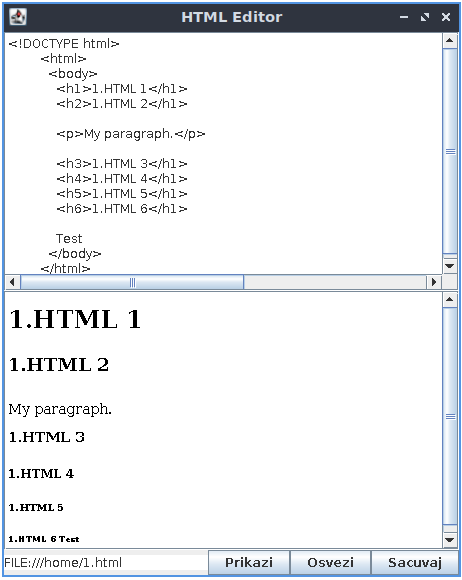
\includegraphics[scale=0.6]{fig.PNG}
  \label{fig2}
\end{figure}


HTML test fajlovi:\\

\noindent
\begin{tabular}{c|c|c}
\begin{lstlisting}
    <!DOCTYPE html>
    <html>
      <body>
        <h1>1.HTML 1</h1>
        <h2>1.HTML 2</h1>
        
        <p>My paragraph.</p>

        <h3>1.HTML 3</h1>
        <h4>1.HTML 4</h1>
        <h5>1.HTML 5</h1>
        <h6>1.HTML 6</h1>

        Test
      </body>
    </html>
\end{lstlisting}&
\begin{lstlisting}
    <!DOCTYPE html>
    <html>
      <body>
        <h1>1.HTML 1</h1>
        <h2>1.HTML 2</h1>
        
        <p>My paragraph.</p>

        <h3>1.HTML 3</h1>

        Test

        <h1>1.HTML 1</h1>
      </body>
    </html>
\end{lstlisting}&
\begin{lstlisting}
    <!DOCTYPE html>
    <html>
      <body>
        Test
        <h2>1.HTML 2</h1>
        <h4>1.HTML 4</h1>
        
        <p>My paragraph.</p>

        <h3>1.HTML 3</h1>

        Test

        <h1>1.HTML 1</h1>
      </body>
    </html>
\end{lstlisting}
\end{tabular} 

\end{document}
